% Handbook Step 2-4 figure snippets generated by scripts/export_handbook_step_figures.py

\begin{figure}[htbp]
  \centering
  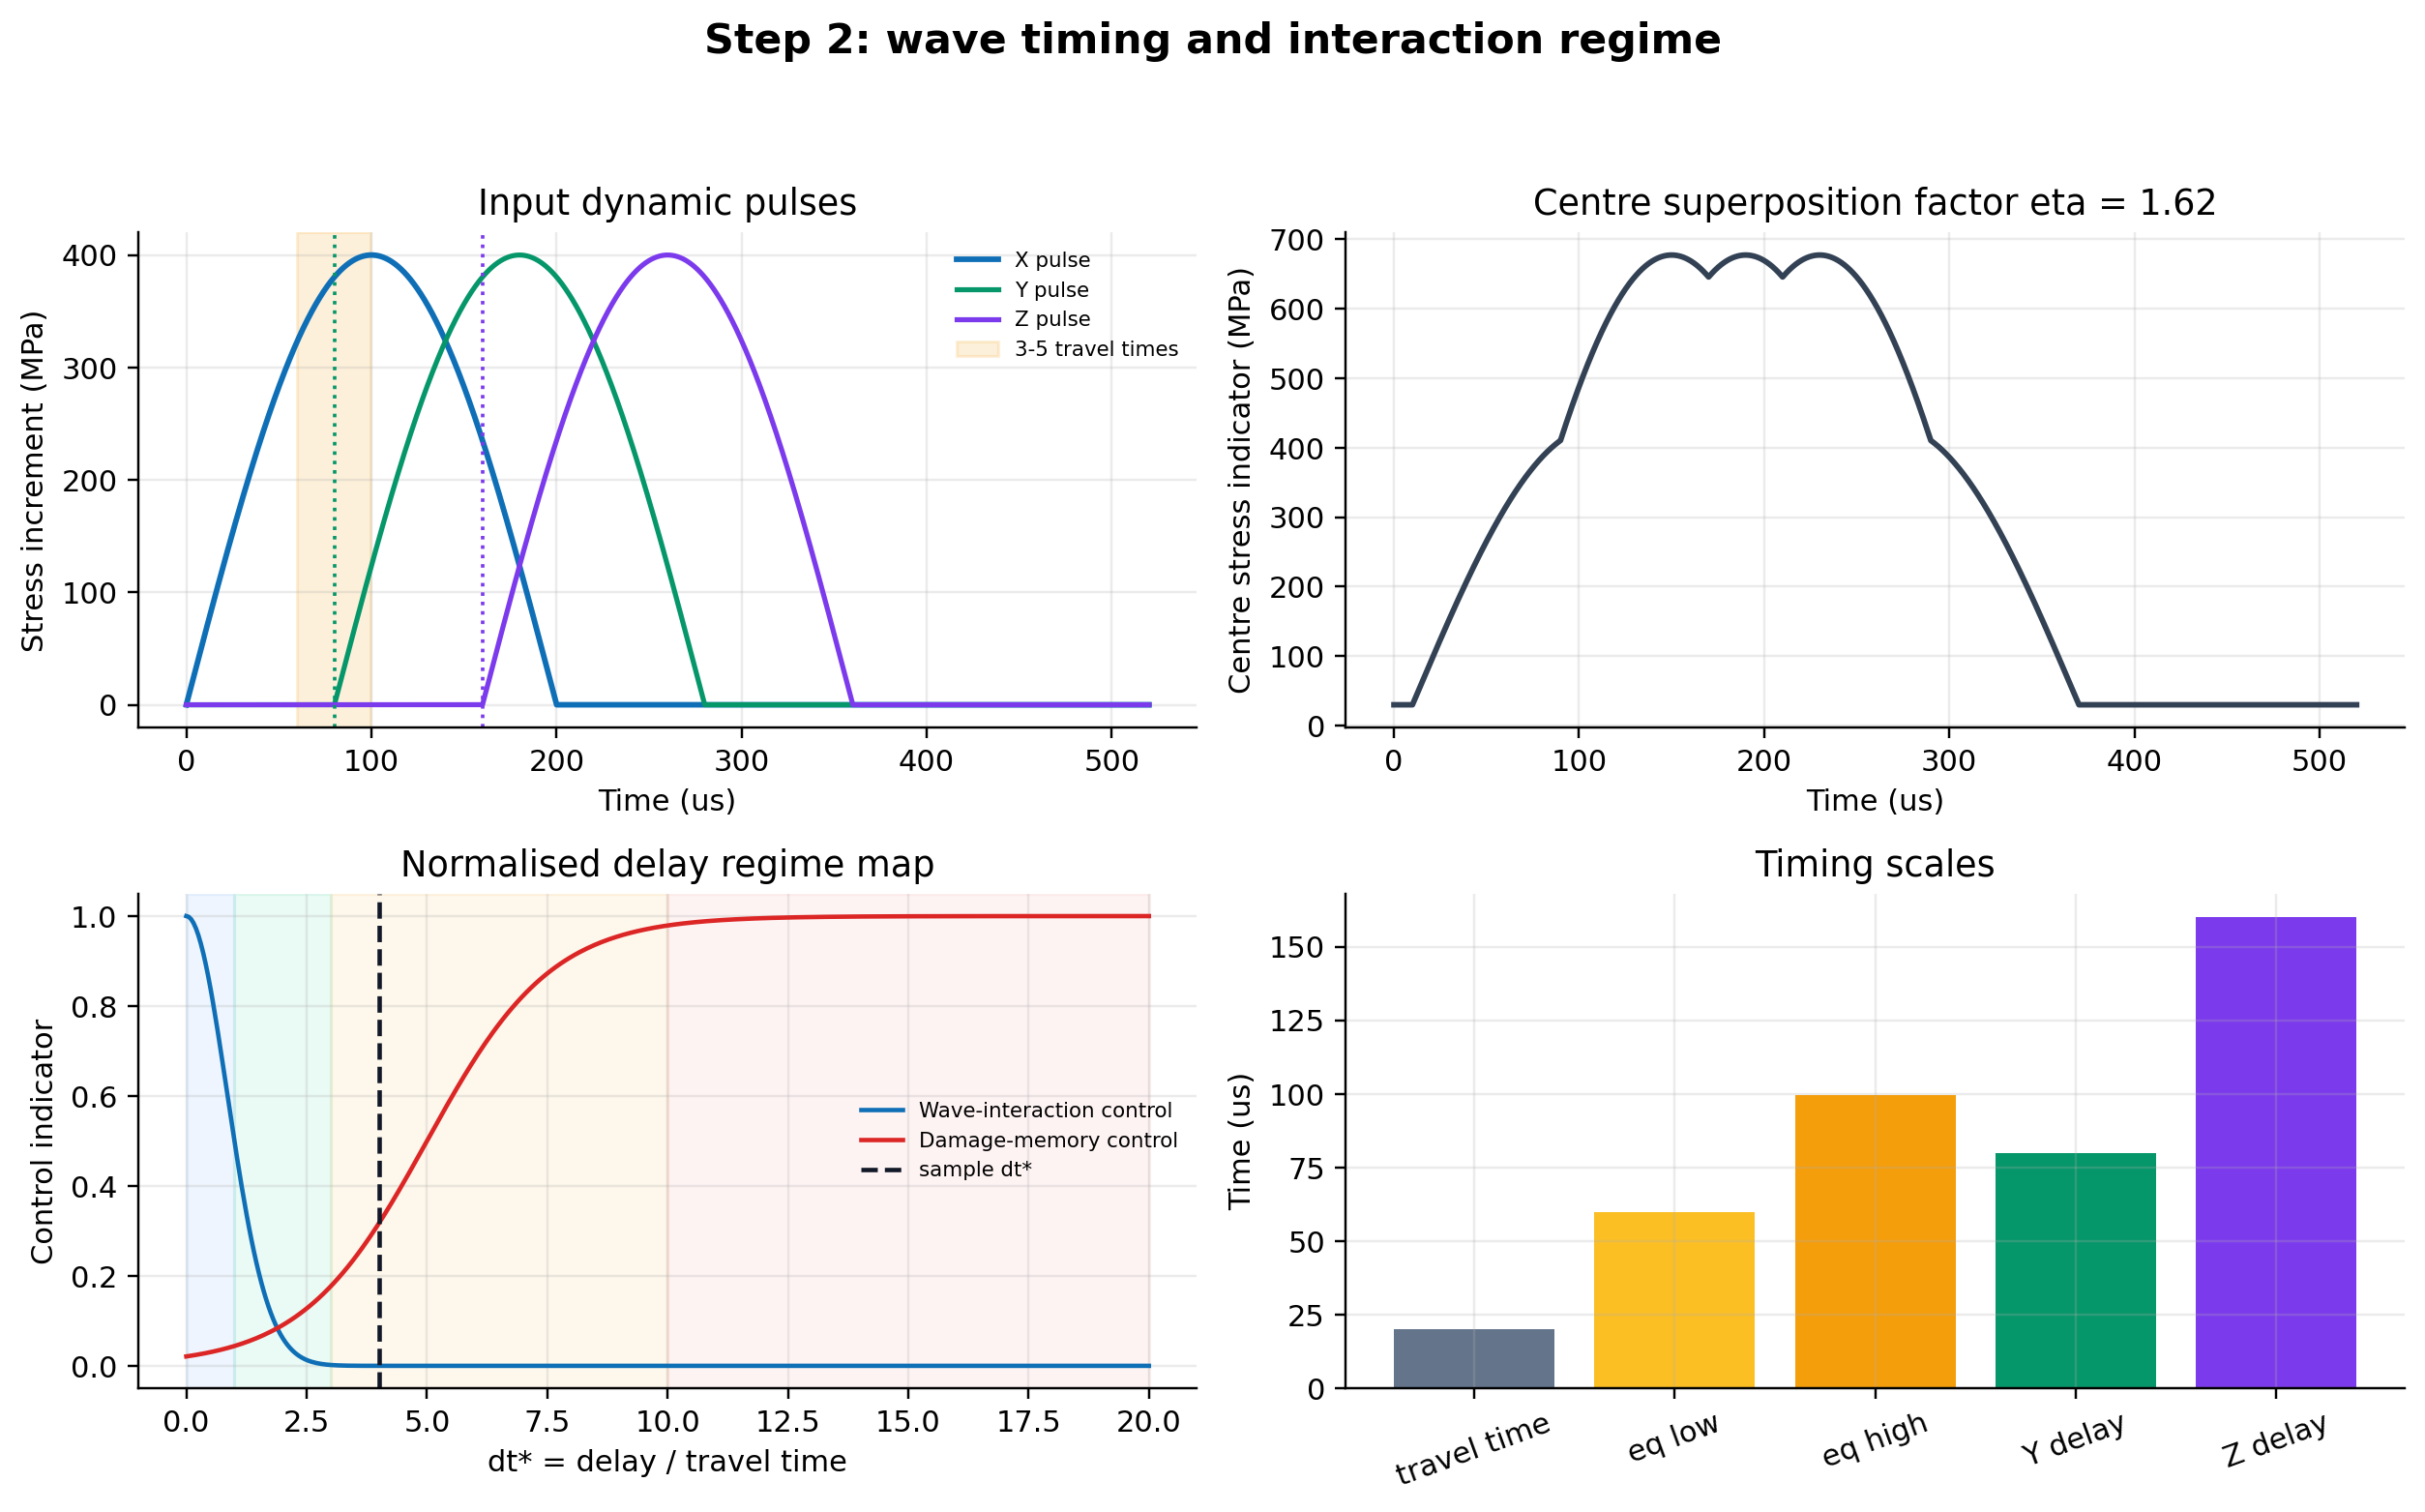
\includegraphics[width=\linewidth]{figures/handbook_steps/step2_wave_timing_regime.png}
  \caption{Step 2 sample wave model for the asynchronous XYZ case: input pulse timing, specimen-centre superposition, normalised delay regime map, and the travel-time/equilibrium scales used by the Streamlit workflow.}
  \label{fig:step2-wave-timing-regime}
\end{figure}

\begin{figure}[htbp]
  \centering
  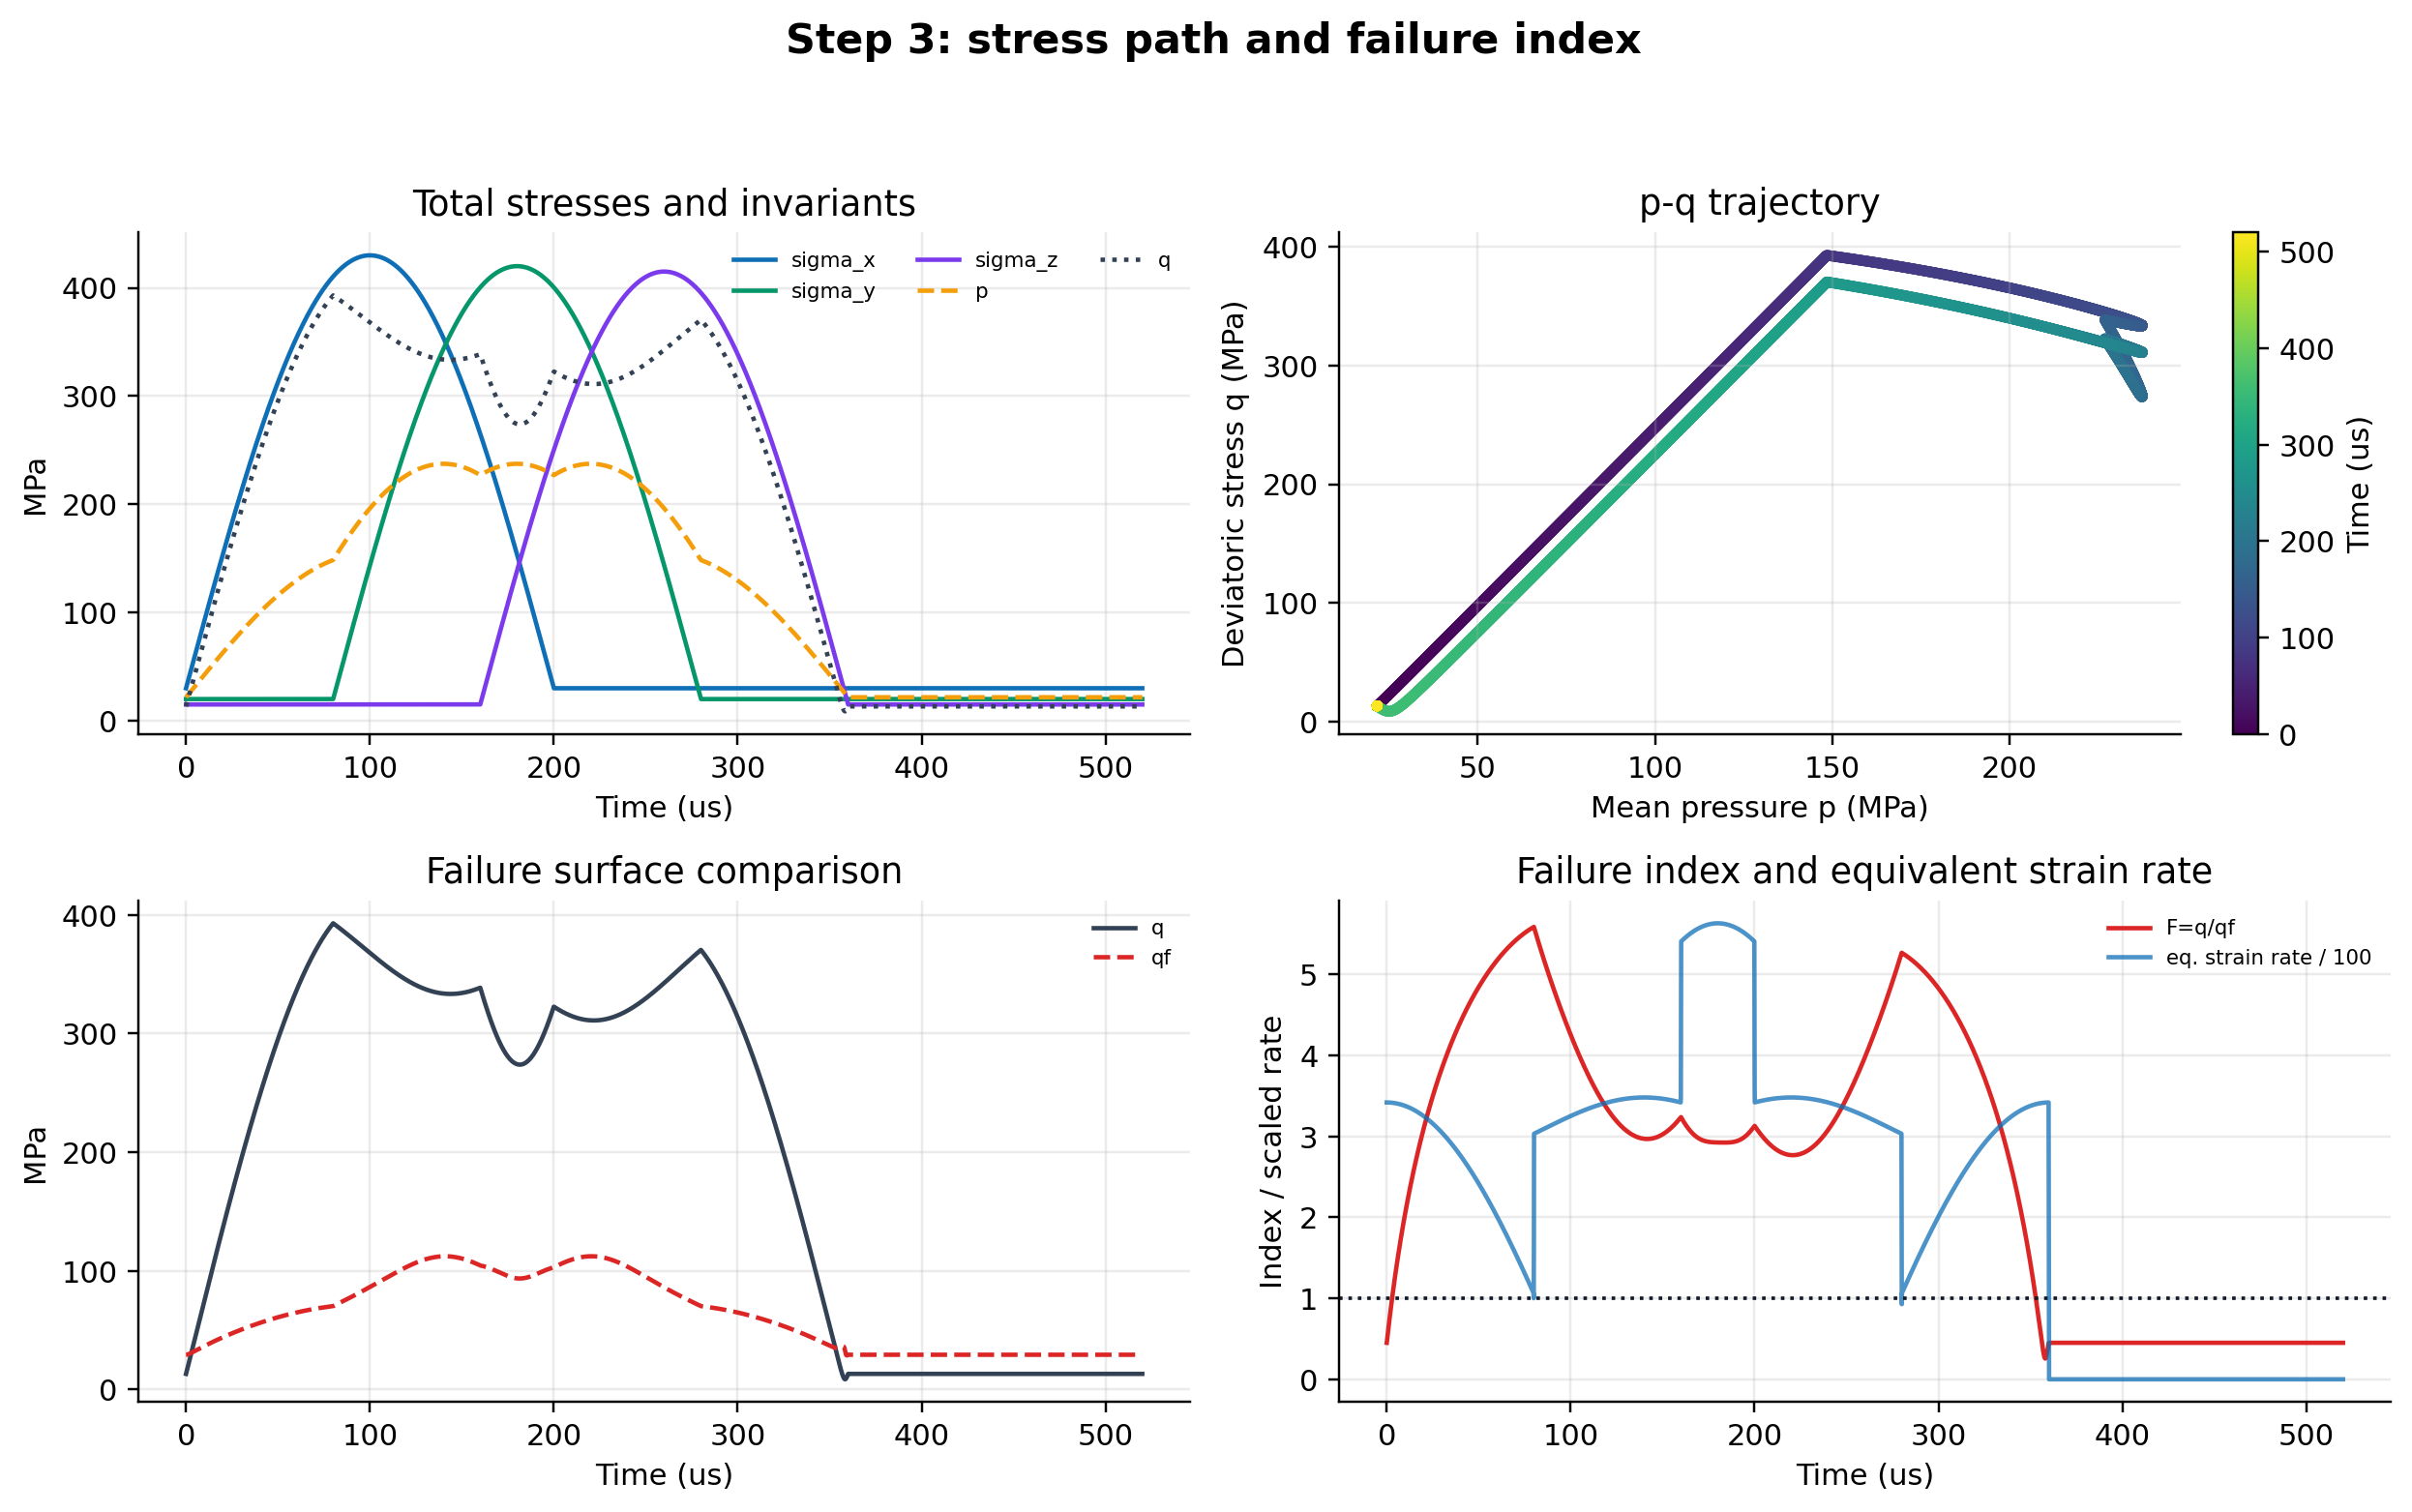
\includegraphics[width=\linewidth]{figures/handbook_steps/step3_stress_path_failure.png}
  \caption{Step 3 sample stress-path analysis: total principal stresses, $p$--$q$ trajectory, comparison of $q$ with the pressure- and Lode-angle-dependent failure surface $q_f$, and the resulting failure index $F=q/q_f$.}
  \label{fig:step3-stress-path-failure}
\end{figure}

\begin{figure}[htbp]
  \centering
  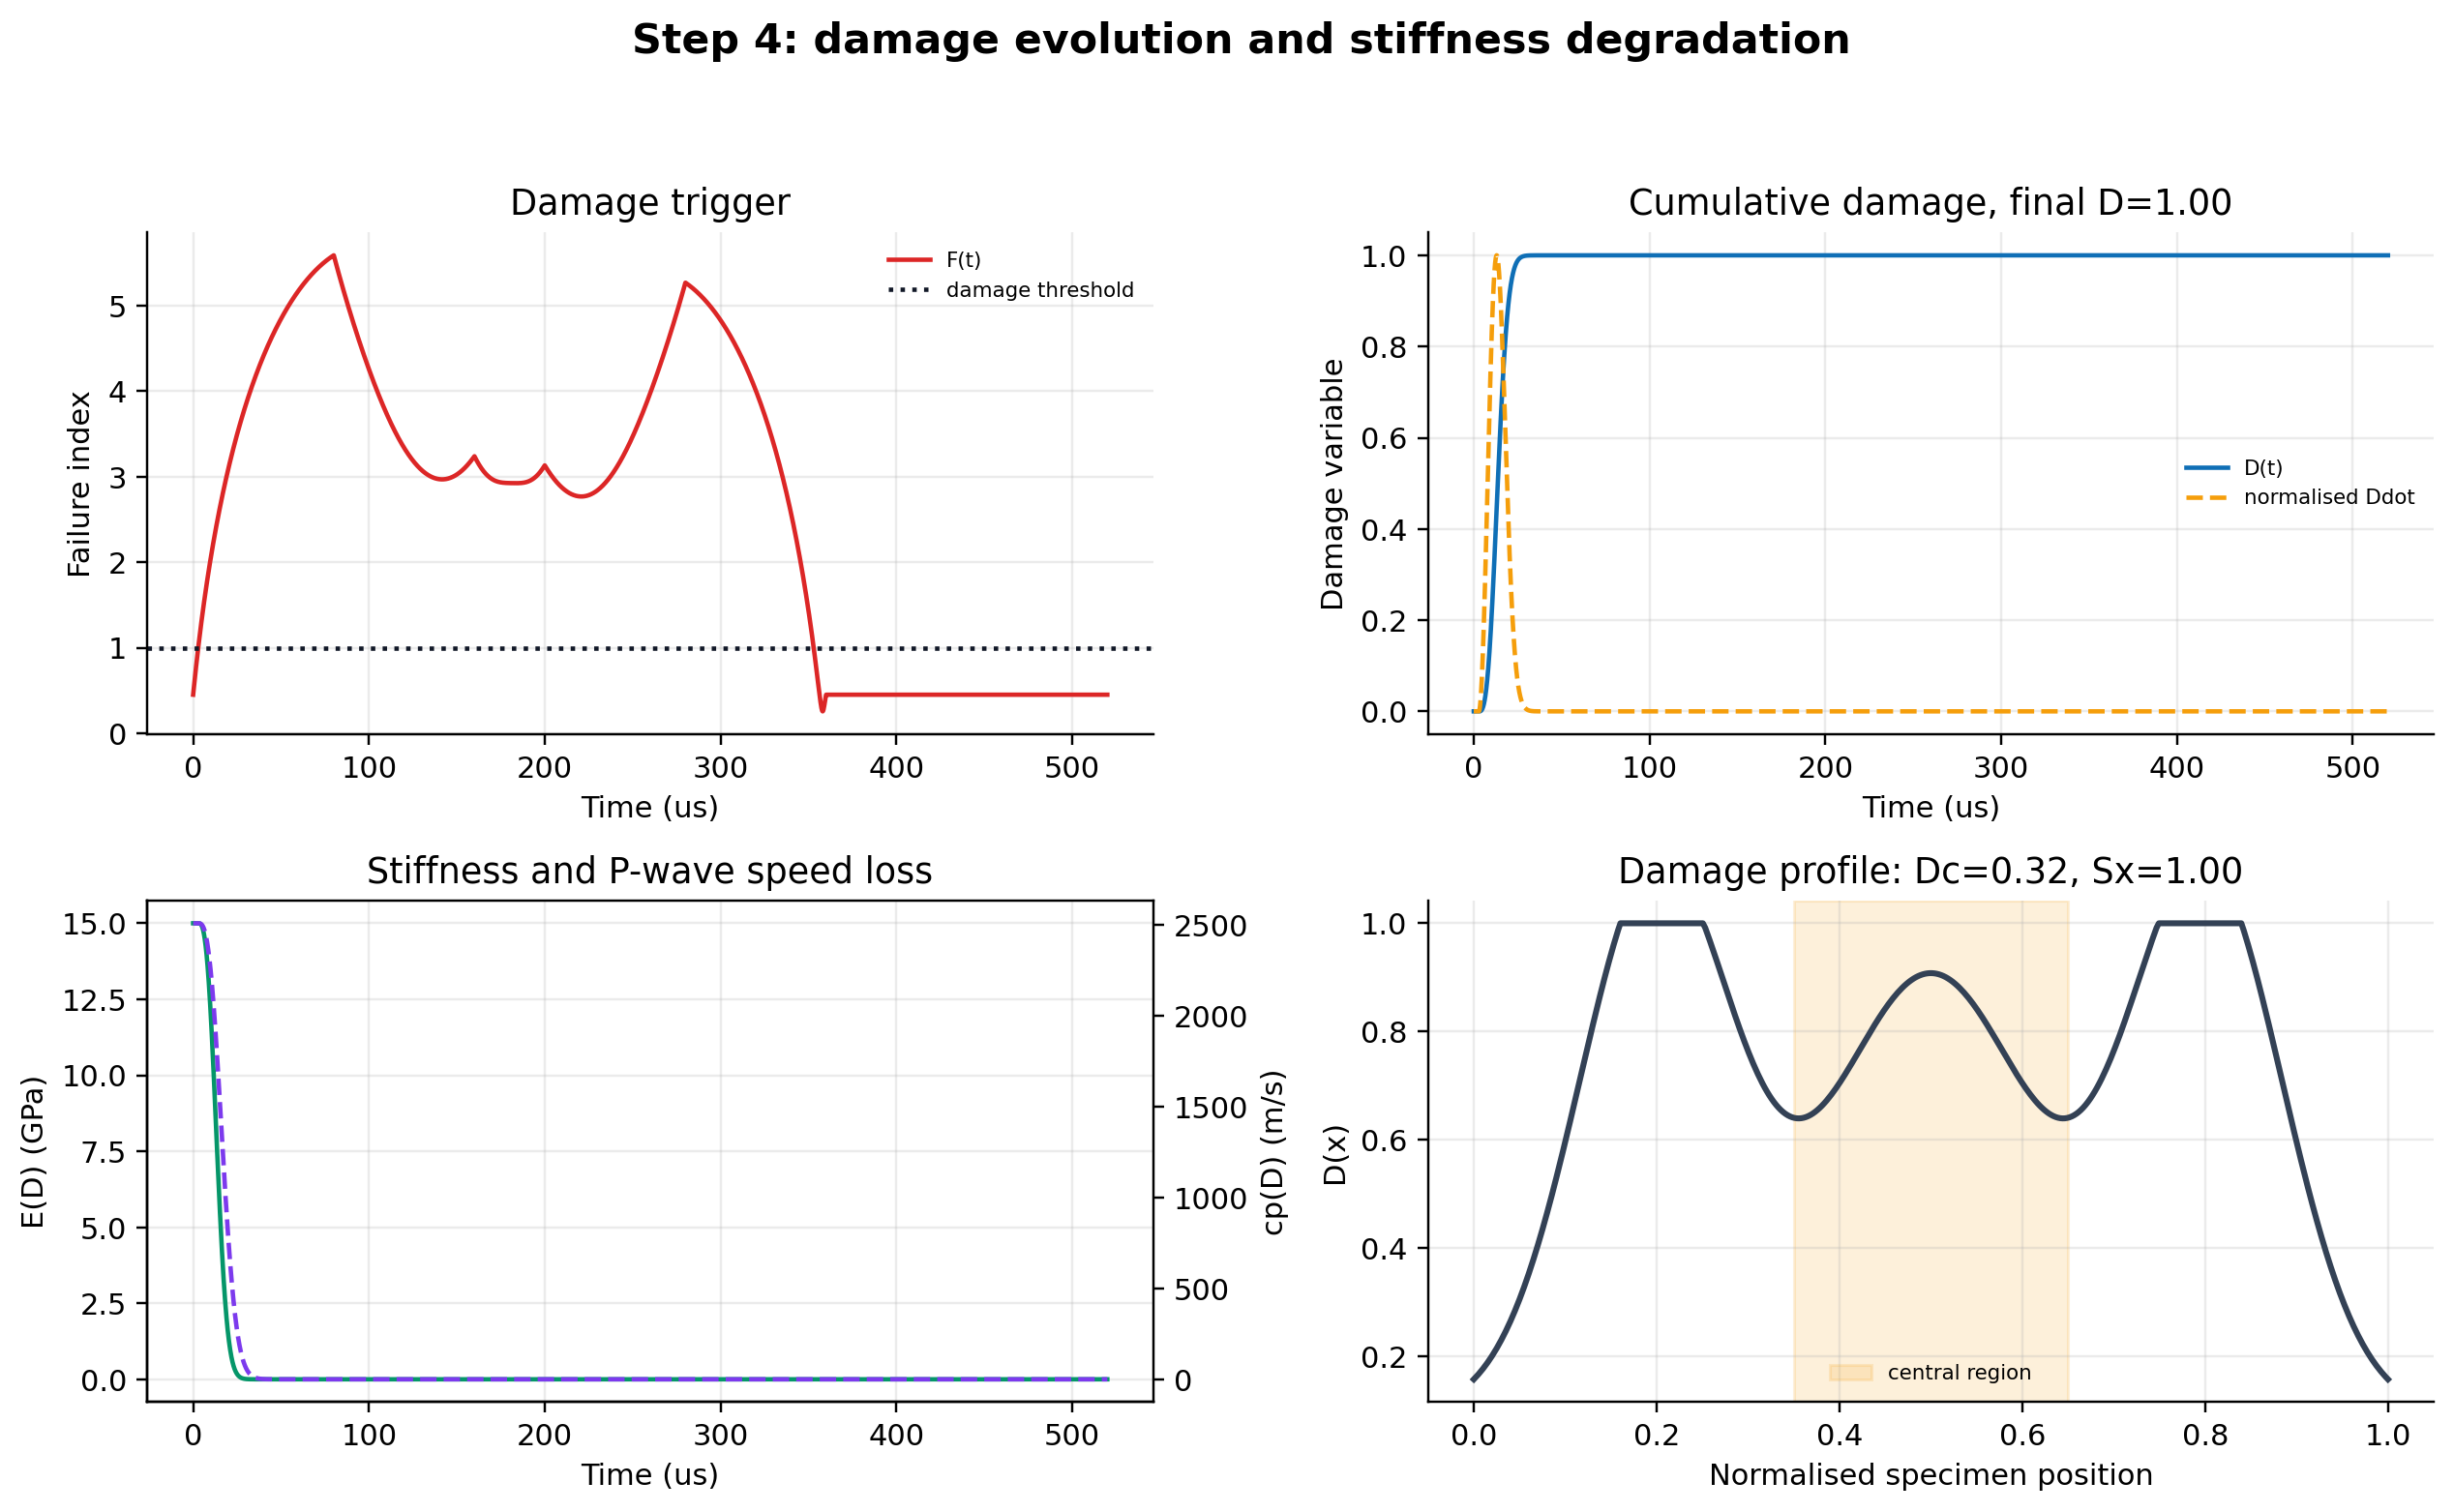
\includegraphics[width=\linewidth]{figures/handbook_steps/step4_damage_evolution.png}
  \caption{Step 4 sample damage analysis: failure-index trigger, cumulative damage and damage rate, stiffness and P-wave-speed degradation, and the synthetic damage-profile descriptors used for DEM/experimental comparison.}
  \label{fig:step4-damage-evolution}
\end{figure}

\begin{figure}[htbp]
  \centering
  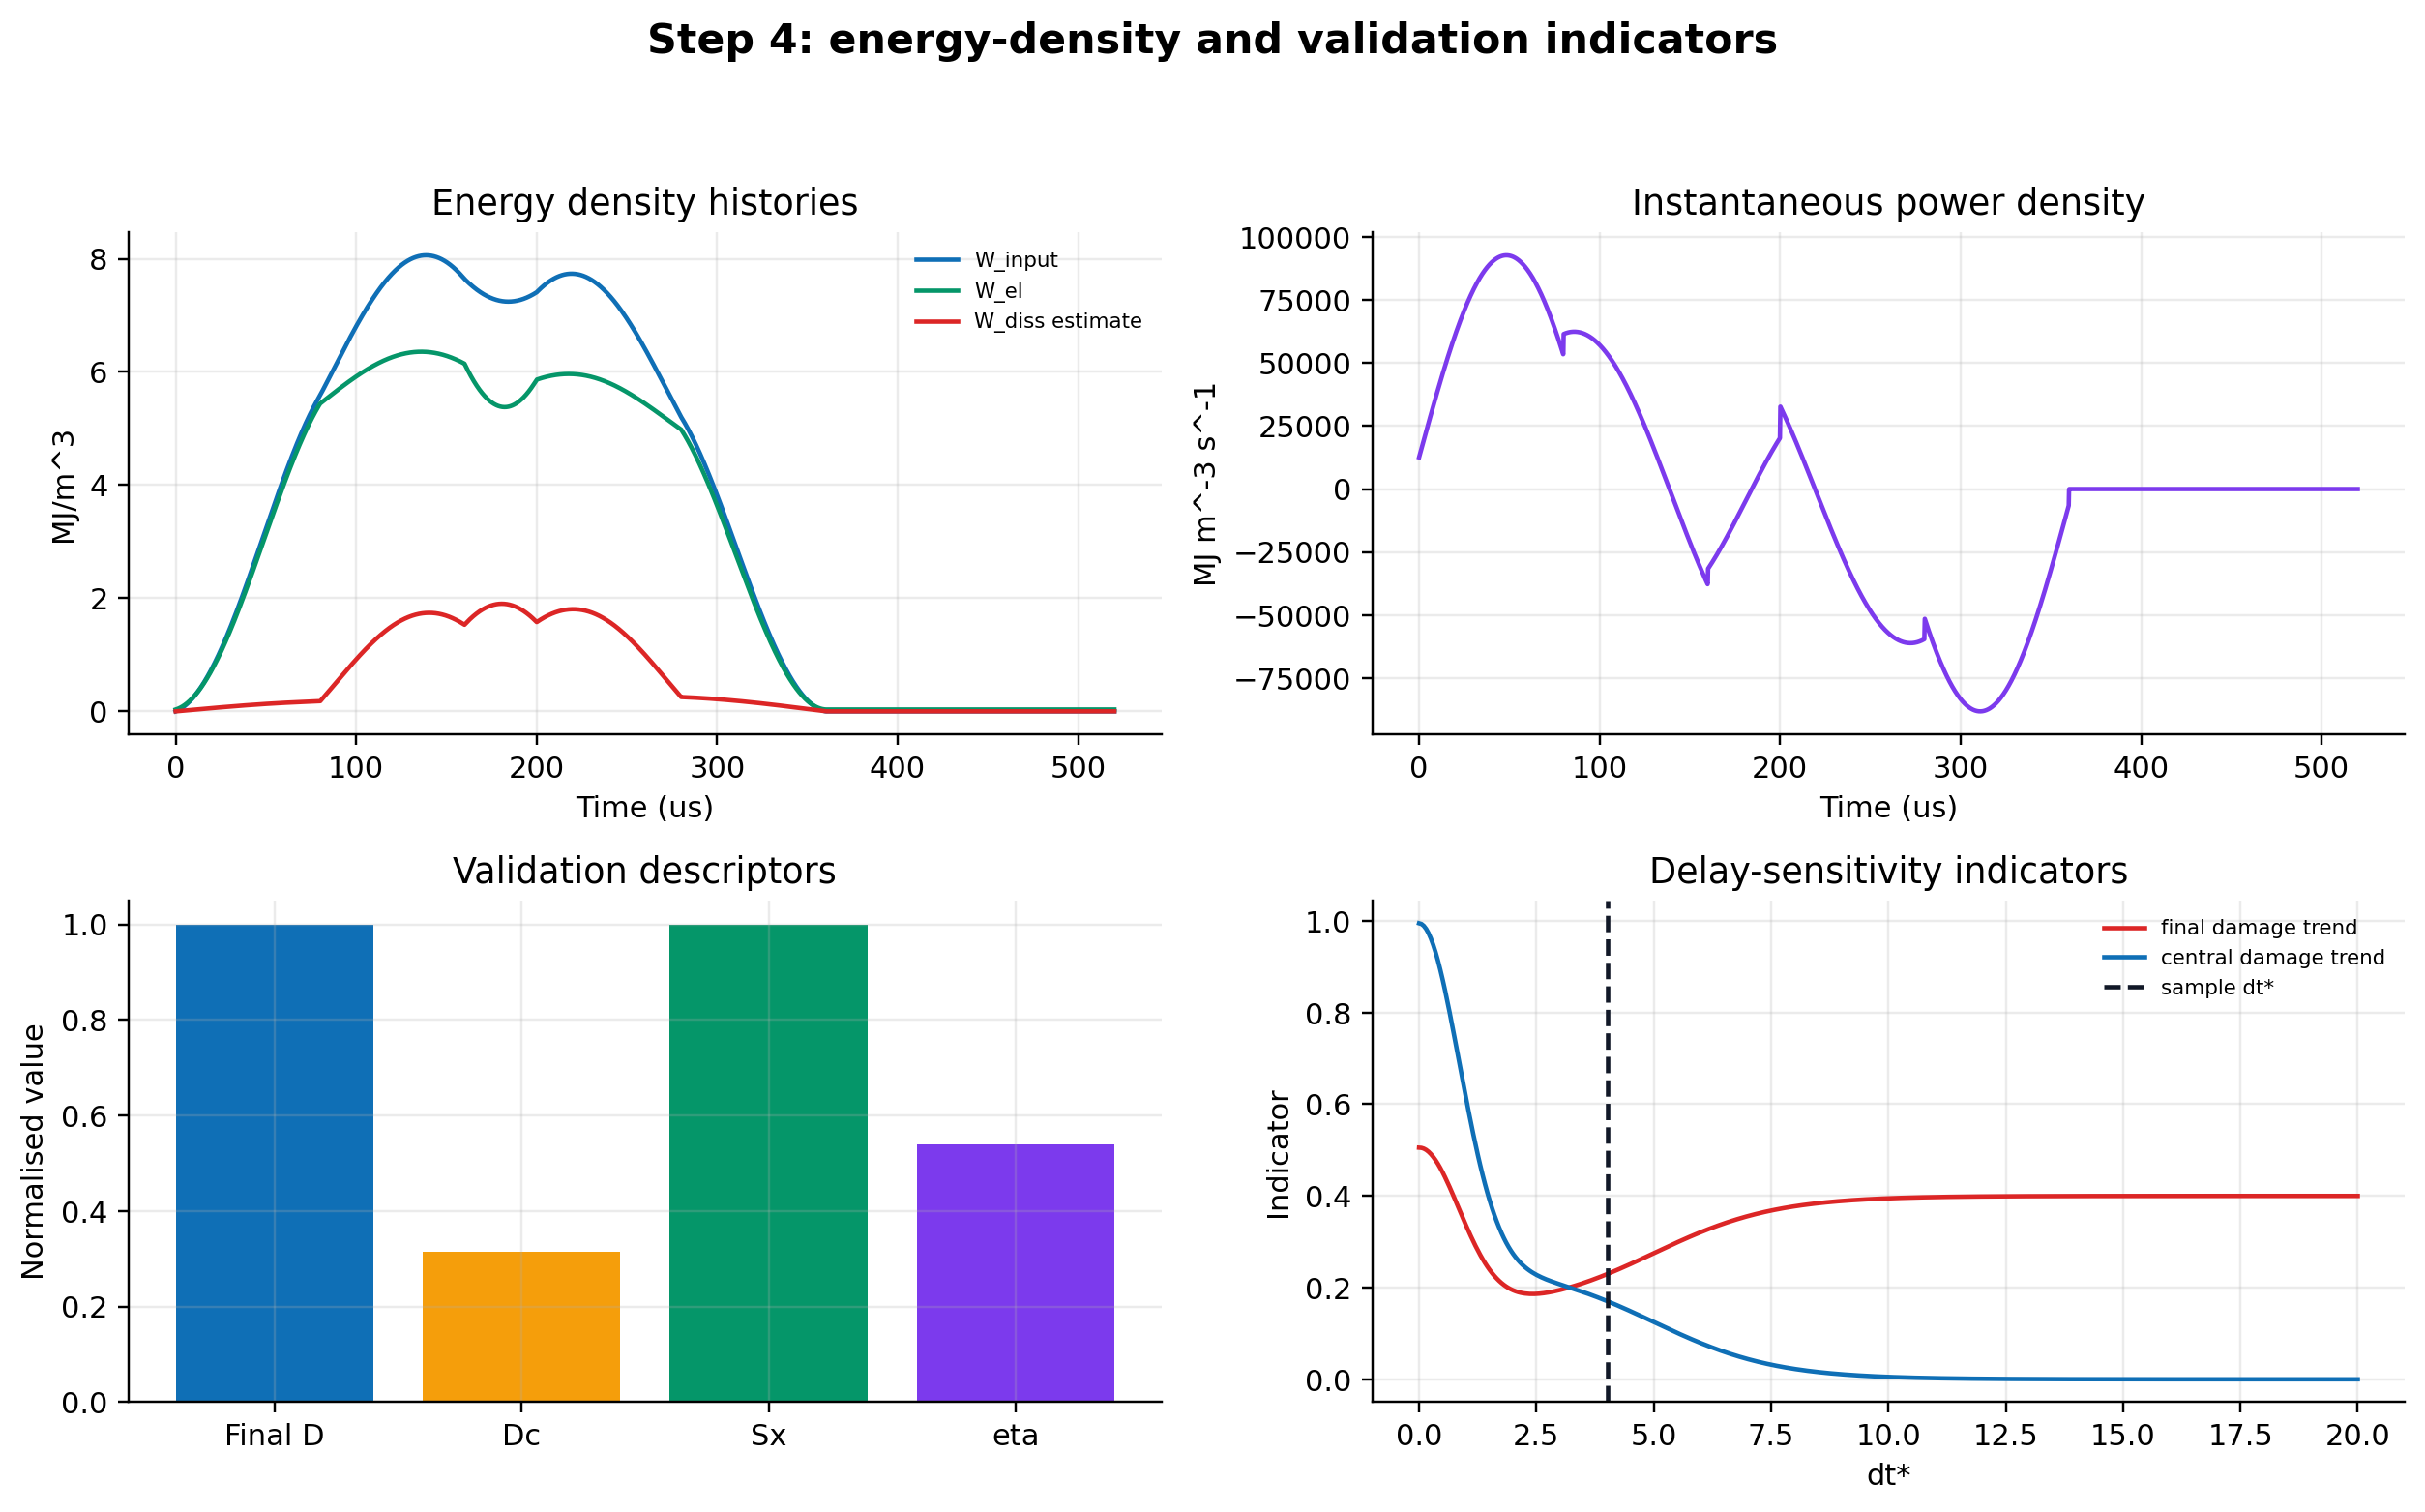
\includegraphics[width=\linewidth]{figures/handbook_steps/step4_energy_density_validation.png}
  \caption{Step 4 sample energy-density and validation view: input, recoverable elastic, and dissipated energy-density estimates, instantaneous power density, scalar validation descriptors, and delay-sensitivity guide curves.}
  \label{fig:step4-energy-density-validation}
\end{figure}
